\section{ Some theoretical basis}
\subsection{What’s deepfake and use?}
 The image or video synthesis technique known as "deepfake" is based on artificial intelligence, more specifically on deep neural networks.  \emph{The term “deepfake” emerged in late 2017 when a redditor (someone who uses reddit platform which is an American social media platform for web content rating by votes along with discussion of websites) posted realistic pornographic videos featuring Hollywood actresses who weren’t really part of it \cite{negiDeepFakeUnderstanding2021} .}Deep fake requires huge data to train models or neural networks to create fake image, video,audios. According to IBM \cite{IBM2023} \emph{Neural networks attempt to mimic the human brain, combining computer science and statistics to solve common problems in artificial intelligence \cite{QuEstceQu}}. A neural network is made up of several layers of neurons, organized into an input layer (which receives the initial data to be processed), one or more hidden layers (which perform complex transformations of the data). Each neuron in these layers applies an activation function to the data received, and an output layer (the final layer produces the results of the network's analysis or prediction). In these layers, each neuron is connected to others, and each connection has an associated weight and threshold.

\begin{figure*}[h]
  \centering
  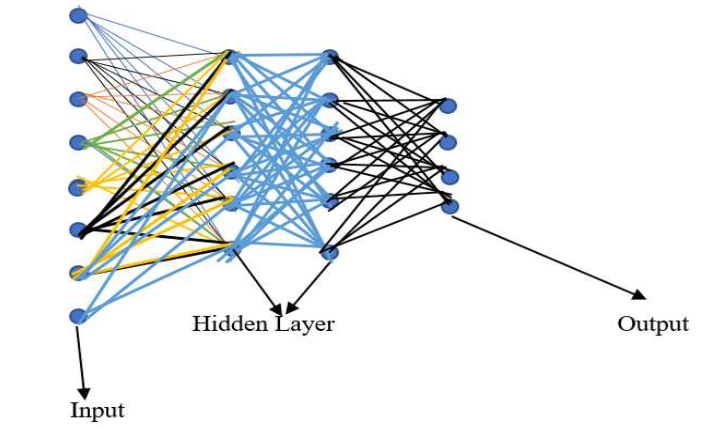
\includegraphics[width=0.7\textwidth]{images/deepNeural.PNG} 
  \caption{Multi layered neuron network \cite{negiDeepFakeUnderstanding2021}}
  \label{fig:your_label}
\end{figure*}
Each artificial neuron receives data, performs a mathematical operation on it using specific weights and thresholds, and then, if the data exceeds a certain threshold, the result is passed on to the next layer. Alternatively, no information is sent at all. Training data helps neural networks adjust their weights and thresholds, improving their ability to perform specific tasks over time. It's an iterative learning process that aims to reduce the number of errors between the network's predictions and expected results.
It is therefore important to say that,\emph{If problem for processing is face generation its more complex because the network has to reads in input and then extract features like eyes, nose, mouth, texture, facial features, determine contort of such features and much more, neural network to generate face should have high processing and a large data and a lot of time as well as complex neural network to understand and train in face recognition \cite{negiDeepFakeUnderstanding2021}.}
\subsubsection{How does deepFake works ?}
Deepfakes work through the use of deep neural networks, in particular adversarial generative networks (AGNs). \emph{A generative adversarial network (GAN) is a machine learning (ML) model in which two neural networks compete with each other by using deep learning methods to become more accurate in their predictions. GANs typically run unsupervised and use a cooperative zero-sum game framework to learn, where one person's gain equals another person's loss.
The two neural networks that make up a GAN are referred to as the generator and the discriminator. The generator is a convolutional neural network and the discriminator is a deconvolutional neural network. The goal of the generator is to artificially manufacture outputs that could easily be mistaken for real data. The goal of the discriminator is to identify which of the outputs it receives have been artificially created \cite{WhatGenerativeAdversarial}.}
The process begins with the collection of massive datasets, typically videos and images of the subject to be reproduced. Two main elements make up the GAN architecture: the generator, which transforms the original subject data to make it similar to the target subject, and the discriminator, which distinguishes between real and generated data. Both elements are trained iteratively at the same time, resulting in a dynamic competition in which the generator constantly improves to deceive the discriminator, and the latter modifies its discernment capabilities. Once the model has been sufficiently trained, the generator is used to create synthetic data, such as an animated face, which can be integrated into an existing video. Post-processing procedures can then be used to enhance the visual quality of the deepfake.

\begin{figure*}[h]
  \centering
  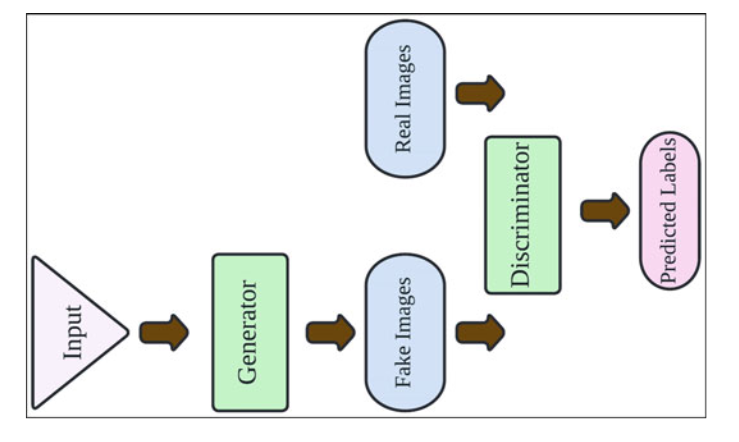
\includegraphics[width=0.7\textwidth]{images/GAN_architecture.PNG} 
  \caption{Architecture of GANs \cite{khanSystematicReviewDeepfake2023}}
  \label{fig:your_label}
\end{figure*}
Deepfakes have given rise to concern because of their potential for misuse, particularly in disinformation and the manipulation of public opinion. \emph{Deep fake can come in use for helping people who have lost their speech to give them new improved voice, commercially deepfake can be used in improving animation or movie quality putting in creative imagination to work as well is therapeutic to people who have lost their dear once. Negative aspects of deep fake include creating fake images, videos, audios that look very real can cause threats to an individual’s privacy, organizations, democracy, and even national security.\cite{negiDeepFakeUnderstanding2021}}